\documentclass[11pt]{aghdpl}
% \documentclass[en,11pt]{aghdpl}  % praca w języku angielskim

% Lista wszystkich języków stanowiących języki pozycji bibliograficznych użytych w pracy.
% (Zgodnie z zasadami tworzenia bibliografii każda pozycja powinna zostać utworzona zgodnie z zasadami języka, w którym dana publikacja została napisana.)
\usepackage[english,polish]{babel}

% Użyj polskiego łamania wyrazów (zamiast domyślnego angielskiego).
\usepackage{polski}

\usepackage[utf8]{inputenc}

% dodatkowe pakiety

\usepackage{mathtools}
\usepackage{amsfonts}
\usepackage{amsmath}
\usepackage{amsthm}

% --- < bibliografia > ---

\usepackage[
style=numeric,
sorting=none,
%
% Zastosuj styl wpisu bibliograficznego właściwy językowi publikacji.
language=autobib,
autolang=other,
% Zapisuj datę dostępu do strony WWW w formacie RRRR-MM-DD.
urldate=iso8601,
% Nie dodawaj numerów stron, na których występuje cytowanie.
backref=false,
% Podawaj ISBN.
isbn=true,
% Nie podawaj URL-i, o ile nie jest to konieczne.
url=false,
%
% Ustawienia związane z polskimi normami dla bibliografii.
maxbibnames=3,
% Jeżeli używamy BibTeXa:
backend=bibtex
]{biblatex}

\usepackage{csquotes}
% Ponieważ `csquotes` nie posiada polskiego stylu, można skorzystać z mocno zbliżonego stylu chorwackiego.
\DeclareQuoteAlias{croatian}{polish}

\addbibresource{bibliografia.bib}

% Nie wyświetlaj wybranych pól.
%\AtEveryBibitem{\clearfield{note}}


% ------------------------
% --- < listingi > ---

% Użyj czcionki kroju Courier.
\usepackage{courier}

\usepackage{listings}
\lstloadlanguages{TeX}

\lstset{
	literate={ą}{{\k{a}}}1
           {ć}{{\'c}}1
           {ę}{{\k{e}}}1
           {ó}{{\'o}}1
           {ń}{{\'n}}1
           {ł}{{\l{}}}1
           {ś}{{\'s}}1
           {ź}{{\'z}}1
           {ż}{{\.z}}1
           {Ą}{{\k{A}}}1
           {Ć}{{\'C}}1
           {Ę}{{\k{E}}}1
           {Ó}{{\'O}}1
           {Ń}{{\'N}}1
           {Ł}{{\L{}}}1
           {Ś}{{\'S}}1
           {Ź}{{\'Z}}1
           {Ż}{{\.Z}}1,
	basicstyle=\footnotesize\ttfamily,
}

% ------------------------

\AtBeginDocument{
	\renewcommand{\tablename}{Tabela}
	\renewcommand{\figurename}{Rys.}
}

% ------------------------
% --- < tabele > ---

\usepackage{array}
\usepackage{tabularx}
\usepackage{multirow}
\usepackage{booktabs}
\usepackage{makecell}
\usepackage[flushleft]{threeparttable}

% defines the X column to use m (\parbox[c]) instead of p (`parbox[t]`)
\newcolumntype{C}[1]{>{\hsize=#1\hsize\centering\arraybackslash}X}


%---------------------------------------------------------------------------

\author{Michał Góra}
\shortauthor{M. Góra}

%\titlePL{Przygotowanie bardzo długiej i pasjonującej pracy dyplomowej w~systemie~\LaTeX}
%\titleEN{Preparation of a very long and fascinating bachelor or master thesis in \LaTeX}

\titlePL{Sterowanie predykcyjne robotem dwukołowym}
\titleEN{Predictive control of two-wheeled robot}


\shorttitlePL{Sterowanie predykcyjne robotem dwukołowym} % %skrócona wersja tytułu jeśli jest bardzo długi
\shorttitleEN{Predictive control of two-wheeled robot}

\thesistype{Praca dyplomowa magisterska}
%\thesistype{Master of Science Thesis}

\supervisor{dr inż. Piotr Bania}
%\supervisor{Marcin Szpyrka PhD, DSc}

\degreeprogramme{Automatyka i Robotyka}
%\degreeprogramme{Computer Science}

\date{2017}

\department{Katedra Informatyki Stosowanej}
%\department{Department of Applied Computer Science}

\faculty{Wydział Elektrotechniki, Automatyki,\protect\\[-1mm] Informatyki i Inżynierii Biomedycznej}
%\faculty{Faculty of Electrical Engineering, Automatics, Computer Science and Biomedical Engineering}

\acknowledgements{Podziękowania }


\setlength{\cftsecnumwidth}{10mm}

%---------------------------------------------------------------------------
\setcounter{secnumdepth}{4}
\brokenpenalty=10000\relax

\begin{document}

\titlepage

% Ponowne zdefiniowanie stylu `plain`, aby usunąć numer strony z pierwszej strony spisu treści i poszczególnych rozdziałów.
\fancypagestyle{plain}
{
	% Usuń nagłówek i stopkę
	\fancyhf{}
	% Usuń linie.
	\renewcommand{\headrulewidth}{0pt}
	\renewcommand{\footrulewidth}{0pt}
}

\setcounter{tocdepth}{2}
\tableofcontents
\clearpage


\chapter{Wprowadzenie}
\label{cha:wprowadzenie}

\section{Cel}

W ramach pracy inżynierskiej powstał dwukołowy robot balansujący. Weryfikacja przyjętych wtedy założeń projektowych uwidoczniła wiele potencjalnych udoskonaleń.

\section{Zakres pracy}

Celem pracy jest budowa robota dwukołowego oraz implemen-
tacja algorytmu predykcyjnego stabilizującego robota w gór-
nym, niestabilnym punkcie równowagi. Konstrukcja mechaniczna będzie bazować na robocie wykonanym w ramach pracy inżynierskiej, zostanei ona przebudowana i dopracowana.

Algorytm będzie rozwiązywał w każdym kroku, odpowiednio sformułowane zadanie
programowania kwadratowego. Jednym z podstawowych elementów pracy będzie też modelowanie oraz identyfikacja modelu matematycznego robota. Algorytm będzie zaimplementowany na platformie STM32F3 Discovery. Zmiana mikrokontrolera wymaga dostosowanie sterownika do pracy w nowych warunkach i napisanie kodu źródłowego. 





\section{Zawartość pracy}
\label{sec:zawartoscPracy}

W rodziale~\ref{cha:pierwszyDokument} przedstawiono....



















\chapter{Konstrukcja mechaniczna}
\label{cha:KonstrukcjaMechaniczna}

W rozdziale zawarto opis konstrukcji ramy pojazdu oraz jednostki napędowej. Założenia projektowe części mechanicznej to uzyskanie maksymalnej trwałości przy utrzymaniu niskich kosztów pojazdu oraz możliwość łatwej modyfikacji i napraw. 

\section{Rama i rozlokowanie podzespołów}
Podstawowym założeniem podczas projektu ramy robota oraz rozlokowywaniu komponentów było zabezpieczenie przed uszkodzeniami wynikającymi z ewentualnych upadków. Rama została wykonana z płyty pleksiglasowej o grubości 4mm. Pozwoliło to utrzymać niską masę przy stosunkowo dużej wytrzymałości konstrukcji. Poszczególne części sterownika zostały przykręcone do ramy w górnej części pojazdu i zabezpieczone przed uderzeniami dodatkowymi fragmentami ramy.

Zastosowanie dwóch kul podporowych, po obu stronach robota, pozwala także na jazdę w pozycji poziomej. Akumulatory zostały umieszczone w dolnej części pojazdu, rozwiązanie to znacznie obniża środek ciężkości. Pozwala to na bardziej dynamiczną jazdę lecz utrudnia stabilizację w górnym punkcie równowagi. W kolejnych podpunktach omówione zostaną kluczowe elementy mechaniczne konstrukcji. Zdjęcie poglądowe robota zostało przedstawione na rysunku \ref{zdj_robot}

\begin{figure}[h]
	\centering
%	\includegraphics[scale=0.6]{}
	\caption{ Zdjęcie poglądowe robota. Zdjęcie własne}
	\label{zdj_robot}
\end{figure}

\section{Silniki}

Jako element napędowy robota zastosowano dwa silniki krokowe 42HS40-0504.Stosunkowo duży moment obrotowy przy niskiej prędkości obrotowej, możliwość kontroli pozycji w pętli otwartej oraz możliwość częstej zmiany kierunku czynią silniki krokowe zasadnym wyborem do pojazdu tego typu. Zastosowane w poprzedniej iteracji projektu silniki zostały jednak wymienione silniki hybrydowe o większym momencie obrotowym oraz wyższej liczbie kroków na obrót. Podstawowe parametry wykorzystanych silników przedstawione zostały w tabeli \ref{tab:skutecznosc}

\begin{table}
	\centering
	
	\begin{tabular}{|c|r|r|}
	
		\hline
		Model& 42HS40-0504 \\		
		\hline
		Liczba kroków&  200\\      
		\hline                                      
		Napięcie znamionowe &12V   \\       
		\hline                                      
		Pobór prądu na cewkę &  0,5A\\ 
		\hline                                                                         
		Rezystancja cewki & 24Ohm\\
		\hline      
		Moment trzymający& 0,44Nm\\
		\hline      
		Wymiary bez wału& 42 x 42 x 40mm\\
		\hline      
		
		\hline        
	\end{tabular}
	\caption{Parametry silników}
	\label{tab:skutecznosc}	
\end{table}



\chapter{Urządzenie elektroniczne}

Rozdział zawiera opis części elektronicznej robota z uwzględnieniem mikro kontrolera, czujników inercyjnych oraz interfejsu mocy do silników krokowych. W dalszych podrozdziałach opisane zostały najważniejsze właściwości użytych podzespołów sterownika oraz sposób ich integracji. 

\section{Sterownik}

Sterownik robota oparty jest o płytkę ewaluacyjną STM32F3 Discovery z mikroprocesorem STM32F303VCT6. Rozwiązanie to udostępnia znaczną moc obliczeniową i pozwala na zastosowanie bardziej zaawansowanych algorytmów sterujących. Najważniejsze cechy modułu STM32F3 Discovery: 

	\begin{tabular}{  l   p{3cm} |}
	-Rdzeń: Cortex M4F \\
	-Taktowanie 72 MHz  \\
	-256 kB Flash \\
	-48kB RAM \\
	-3- osiowy, cyfrowy żyroskop L3GD20 \\
	-3- osiowy, cyfrowy akcelerometr z magnetometrem LSM303DLHC \\
	-10 diod LED  \\
	-Dwa przyciski 		 \\	
\end{tabular}  




Wykorzystanie elementów umieszczonych na płytce ewaluacyjnej pozwala zredukować wykorzystanie dodatkowych podzespołów o niezbędne w projekcie czujniki inercyjne oraz ułatwiające proces projektowy diody i przyciski. Schemat demonstrujący sposób komunikacji podzespołów sterownika znajduje się na rysunku \ref{schemat}



\begin{figure}[h]
	\centering
	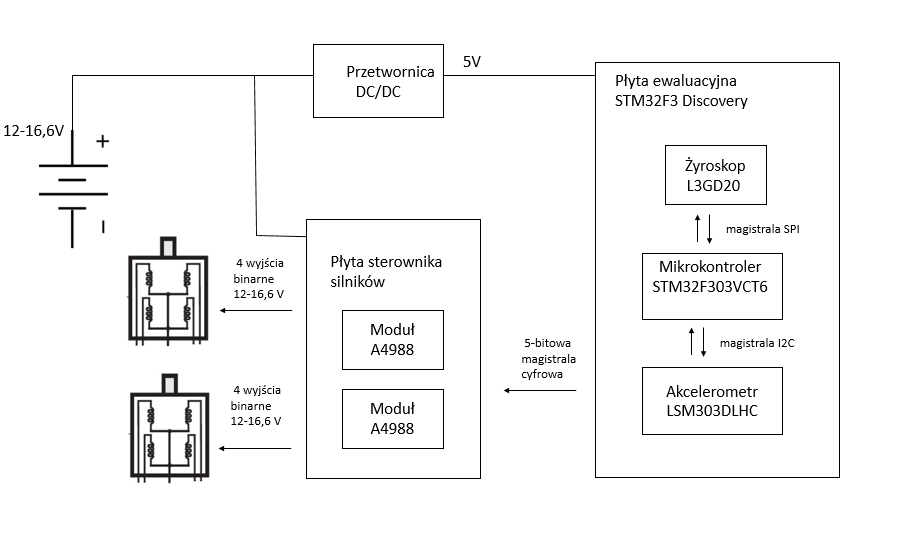
\includegraphics[scale=0.6]{schemat_sterownika.png}
	\caption{ Schemat steroniwka. Grafika własna}
	\label{schemat}
\end{figure}


\section{Żyroskop}

Wykorzystane żyroskop to zawarty na płytce ewaluacyjnej układ L3GD20. Jest to trójosiowy żyroskop cyfrowy. Jego kluczowe właściwości to:

\begin{tabular}{  l   p{3cm} |}
	 -Trzy dostępne skale pomiarowe (250/500/2000 dps) \\
	 -Interfejs komunikacyjny $I^2C$ lub $SPI$\\
	-16 bitowa rozdzielczość pomiarów \\
\end{tabular}  

W projekcie komunikacja z czujnikiem przebiega przy użyciu protokołu SPI. Wykorzystywana skala pomiarowa to: 500 dps.


\section{Akcelerometr}
Kolejnym wykorzystanym elementem płytki ewaluacyjnej jest trójosiowy akcelerometr z magnetometrem LSM303DLHC. 

\begin{tabular}{  l   p{3cm} |}
	- Interfejs komunikacyjny: I2Cm\\
	-Akcelerometr, zakres: $\pm$ 2 g, $\pm$ 4 g, $\pm$ 8 g oraz $\pm$ 16 g\\
	-Magnetometr, zakres:  od $\pm$ 1,3 do $\pm$ 8,1 gauss\\
	-16 bitowa rozdzielczość pomiarów \\
\end{tabular}  


Sensor został skonfigurowany na zagres $\pm$2g. Mangetometr nie został wykorzystany ze względu na znaczne zakłócenia wskazań poprzez niewielką odległość od silników .


\section{Sterownik silników krokowych}

Do kontroli silników krokowych wykorzystany został sterownik stworzony na potrzeby pracy inżynierskiej. Jest on oparty o 2 układy A4988, każdy z nich pozwala sterować pojedyńczym silnikiem za pomocą dwóch wyprowadzeń cyfrowych.Zbocze narastające na drugim powoduje wykonanie kroku w kierunku ustawionym przez stan drugiego wyprowadzenia. Sterowniki pozwalają na sterowanie mikrokrowoe w trybie 1/2, 1/4, 1/8 i 1/16 kroku. W projekcie silniki zostały skonfigurowanę na pracę w trybie 1/8 kroku, pojedyńczy krok w tym trybie obraca wał o 0.225 stopnia.  Ustawienie to dostarcza wystarczającą precyzję sterowania. Użycie pracy w trybie 1/16 kroku zmniejszyłoby moment oborotowy silników a dalsze zwięszkanie precyzji sterowania nie jest konieczne.


\section{Zasilanie}

Robot jest zasilany przy pomocy 4 ogniw litowo-jonowych połączonych szeregowo. Są to niezależne ogniwa 18650 o napięciu znamionowym 3.7V i pojemności około 2200mAh. Napięcie całego pakietu waha się od 16.8V przy pełnym naładowaniu do 12V w stanie rozładowania akumulatorów. Elektronika zasilana jest przy pomocy regulowanej przetwornicy impulsowej dostarczającej napięcie 5V. Sterownik silników zasilany jest bezpośrednio z akumulatorów w związku z czym ich zachowanie zależne jest od stopnia rozładowania.



\newcommand{\Lagr}{\mathcal{L}}
\chapter{Modelowanie i identyfikacja}
\label{cha:model}

Wstępne obliczenia matematyczne oraz symulacje są ważnym elementem procesu projektowego umożliwiającym wczesną weryfikację przyjętych założeń. Model matematyczny oparty o wstępnie oszacowany parametry umożliwia przetestowanie projektu przed zużyciem czasu i środków na potencjalnie błędne rozwiązanie. 

\section{Model nieliniowy}
\label{nieliniowy}

Model matematyczny robota bazuje na nieliniowych równaniach różniczkowych uzyskanych przy pomocy równań Lagranga. Wyprowadzenie zostało w pełni oparte o [X] oraz zweryfikowane przy pomocy symulacji opisanej w punkcie X.X. 

\subsection{Opis matematyczny obiektu}

Przyjęte założenia: oba koła poruszają się z tą samą prędkością obrotową bez poźligu między powierzchnią koła a podłożem.

Zmienne opisujące system:


	\begin{tabular}{  l l  p{3cm} |}
		$x$& - pozioma odległość środka koła od przyjętego układu współrzędnych\\ 
		$x_c$& - pozioma odległość środka masy od przyjętego układu współrzędnych\\ 
		$z_c$& - pionowa odległość środka masy od przyjętego układu współrzędnych\\ 
		$\phi$& - położenie kątowe koła\\ 
		$\theta$& - położenie kątowe robota względem pozycji pionowej\\ 			
	\end{tabular}  



Pozostałe parametry to:


	\begin{tabular}{  l l  p{3cm} |}
		$m$& - Masa korpusu robota\\ 
		$m_w$& - Masa kół\\ 
		$R$& - Promień koła\\ 
		$L$& - Odległość pomiędzy środkiem masy a osią koła\\ 
		$\tau_0$& - zastosowany moment obrotowy\\ 
		$I$& - moment bezwładność korpusu robota\\ 
		$I_w$& - moment bezwładność kół 		\\ 	
	\end{tabular}  



Wizualizacja przyjętych symboli została przedstawiona na rysunku \ref{fig:img4_01}

\begin{figure}[h]
	\centering
	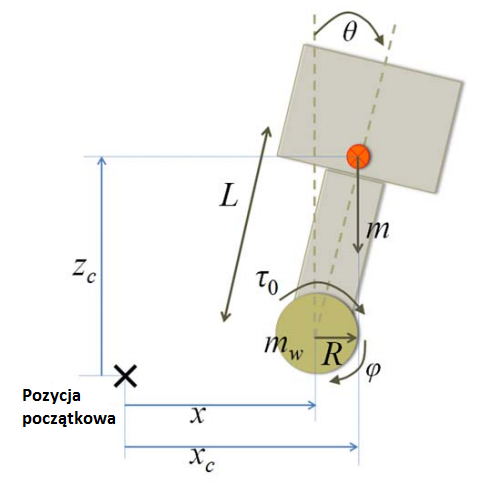
\includegraphics[scale=0.6]{img4_01.png}
	\caption{Przyjęty opis stanu obiektu}
	\label{fig:img4_01}
\end{figure}


\subsubsection{Wyprowadzenie równań modelu}
\label{wypr_rownan}
Zmienne $x, x_c, \dot{x}, \dot{x_c}, \dot{z_c} $ można zapisać jako:

\begin{equation}   x=R \phi  
\label{4row01}      \end{equation}
\begin{equation}   x_c=R \phi +Lsin\theta        \end{equation}
\begin{equation}   z_c=R +Lcos\theta       \end{equation}
\begin{equation}    \dot{x}= R \dot{\phi}      \end{equation}
\begin{equation}     \dot{x_c}= R \dot{\phi} + L\dot{\theta}cos\theta    \end{equation}
\begin{equation}  \dot{z_c}=-L\dot{\theta}sin\theta   
\label{4row06}       \end{equation}


Na podstawie równań \ref{4row01}:\ref{4row06} możemy zapisać energię potencjalną $E_p$ i kinetycznę $E_p$ w postaci \ref{4row07}:\ref{4row10}

\begin{equation}    
\label{4row07}     
E_p=mg(R+Lcos\theta)-mg(R+L)=mgl(cos\theta-1)
 \end{equation}
 \begin{equation}  E_k=1/2 m_w\dot{x}^2+1/2 I_w \dot{\phi}^2+1/2m\dot{x}_c^2+1/2m\dot{z}_c^2 +1/2mI\dot{\theta}^2   
  \end{equation}
\begin{equation} 
\label{4row10}    
 =1/2(I_w+m_wR^2+mR^2)\dot{\phi}^2 +mRLcos\theta \dot{\phi}\dot{\theta}+1/2*(I+mL^2)\dot{\theta}^2
\end{equation}

Lagranżian  $\Lagr$ może być zapisany jako różna pomiędzy energią kinetyczną a potencjalną

\begin{equation} 
\Lagr=E_k-E_p
\end{equation}
\begin{equation} 
=1/2(I_w+m_wR^2 +mR^2)\dot{\phi}^2 +mRLcos\theta\dot{\phi}\dot{\theta}+
1/2(I+mL^2)\dot{\theta}^2 +mgL(cos\theta-1)
\end{equation}

W związku z czym równania dynamiczne dla składowych $\theta$ i $\phi$ mogą zostać wyznaczone w \ref{4row11}:\ref{4row12}

\begin{equation} 
\label{4row11}    
\dfrac{\partial \Lagr}{\partial \dot{\phi}}=(I_w+m_wR^2+mR^2)\dot{\phi}+mRL\dot{\theta}cos\theta
\end{equation}
\begin{equation} 
\dfrac{\partial \Lagr}{\partial \phi}=0
\end{equation}
\begin{equation} 
\dfrac{d}{dt}(\dfrac{\partial \Lagr}{\partial \dot{\phi}})-\dfrac{\partial \Lagr}{\partial \phi}=
(I_w +m_w R^2 +mR^2)\ddot{\theta}+mRLcos\theta\ddot{\theta}-mRLsin\theta\ddot{\theta}^2=\mu
\end{equation}




\begin{equation} 
\dfrac{\partial \Lagr}{\partial \dot{\theta}}=mRLcos\theta\dot{\phi}+(I+mL^2)\dot{\theta}
\end{equation}

\begin{equation} 
\dfrac{\partial \Lagr}{\partial \theta}=-mRLsin\theta\dot{\phi}\dot{\theta}+mgLsin\theta
\end{equation}
\begin{equation} 
\label{4row12}  
\dfrac{d}{dt}(\dfrac{\partial \Lagr}{\partial \dot{\theta}})-\dfrac{\partial \Lagr}{\partial \theta}=
(I+mL^2)\ddot{\theta}+mRLcos\theta\ddot{\phi}-mRLsin\theta=\chi
\end{equation}

Gdzie $\mu$ i $\chi$ to uogólnione siły(momenty obrotowe) dla odpowiednich składowych.
Uzyskane w ten sposób równania różniczkowe można zapisać w postaci macierzowej 


\begin{equation}
\label{4row13} 
\begin{bmatrix} {I_w+(m_w+m)R^2} & {mRLcos \theta} \\{mRLcos\theta} & {I+mL^2} \end{bmatrix}
\begin{bmatrix}	\ddot{\phi}  \\	\ddot{\theta}  \end{bmatrix} +
\begin{bmatrix}	0 &-mRLsin\theta\dot{\theta} \\	0 &0 \end{bmatrix} 
\begin{bmatrix}	\dot{\phi}  \\	\dot{\theta} \end{bmatrix} +
\begin{bmatrix}	{0}  \\	{-mgLsin\theta}  \end{bmatrix} =
\begin{bmatrix}	{\mu}  \\	{\chi} \end{bmatrix}  
\end{equation}

Kolejny krok skupia się na wyrażeniu uogólnionych momentów obrotowych za pomocą znanych parametrów. Mommeny obrotowy działający na robota możemy zapisać jako sumę momentów wytworzonych przez silniki oraz rozproszonych poprzez tarcie. 


	\begin{tabular}{  l l  p{3cm} |}
	$ \tau_0 $& - łączny moment obrotowy dostarczony przez silniki \\ 
	$ \tau_a $  & -moment rozproszony poprzez tarcie w łożyskach \\ 
	$ \tau_f $  & -moment rozproszony poprzez tarcie kół o podłoże \\ 	
	$ \beta_a $  & -współczynnik tarcia w łożyskach \\ 	
	$ \beta_f $  & -współczynnik tarcia kół o podłoże \\ 	
\end{tabular}  

Po wprowadzeniu powyższych parametrów możemy zapisać uogólnione momenty obrotowe w postaci \ref{4row14}:\ref{4row15}

\begin{equation}
\label{4row14} 
\mu=\tau_0-\tau_a-\tau_f = \tau_0 -\beta_f(\dot{\phi}-\dot{\theta})-\beta_a\dot{\phi}
\end{equation}
\begin{equation}
\label{4row15} 
\chi=-\tau_0+\tau_a=-\tau_0+\beta_f(\dot{\phi}-\dot{\theta})
\end{equation}







\section{Model liniowy}

Kontrola predykcyjna opiera się na modelu liniowym wyrażonym równaniami stanu. Wprowadzony w punkcie \ref{nieliniowy} model robota jest nieliniowy, w związku z czym, wymaga on linearyzacji w punkcie równowagi. Jako punkt linearyzacji modelu wybrany został górny, niestabliny punkt równowagi.

Do w celu umożliwienia linearyzacji koniecznie były następujące uproszczenia:
\begin{itemize}
	\item  Niewielki zakres ruchów względem pozycji pionowej 
	\item  $cos\theta \approx 1$
	\item  $sin\theta \approx 0$
\end{itemize}

Równania modelu \ref{4row14} po wprowadzeniu tej modyfikacji przedstawione zostały jako równanie \ref{4row16}.

\begin{equation}
\label{4row16} 
\begin{bmatrix} {I_w+(m_w+m)R^2} & {mRL} \\{mR} & {I+mL^2} \end{bmatrix}
\begin{bmatrix}	\ddot{\phi}  \\	\ddot{\theta}  \end{bmatrix} +
\begin{bmatrix}	\beta_a + \beta_f &-\beta_f \\	-\beta_f &\beta_f \end{bmatrix} 
\begin{bmatrix}	\dot{\phi}  \\	\dot{\theta} \end{bmatrix} +
\begin{bmatrix}	{0}  \\	{-mgL}  \end{bmatrix}\theta =
\begin{bmatrix}	{1}  \\	{-1} \end{bmatrix}  \tau_0
\end{equation}


Równanie \ref{4row16} można przedstawić w zwięzłym stylu w postaci \ref{4row18}

\begin{equation}
\label{4row18} 
E
\begin{bmatrix}	\ddot{\phi}  \\	\ddot{\theta}  \end{bmatrix} +
F
\begin{bmatrix}	\dot{\phi}  \\	\dot{\theta} \end{bmatrix} +
G\theta
=H\tau_0
\end{equation}

Na postawie równania \ref{4row18} możemy zapisać model systemu w postaci równań stanu. Jako zmienne stanu wykorzystane zostaną $\phi, \theta, \dot{\phi}, \dot{\theta}$. Wejściem systemu jest moment obrotowy $\tau_0$. Jako wyjścia zostały wybrane przemieszczenie robota w osi $x$ oraz położenie kątowe korpusu $\theta$. W związku z tymi założeniami równania stanu systemu przyjmują postać  \ref{4row19} :\ref{4row20} 

\begin{equation}
\label{4row19} 
\frac{d}{dt}
\begin{bmatrix}	\phi \\ \theta \\ \dot{\phi}  \\	\dot{\theta}  \end{bmatrix} 
=
TO_DUZE
\begin{bmatrix}		\phi \\ \theta \\\dot{\phi}  \\	\dot{\theta} \end{bmatrix} +
\begin{bmatrix}	0 \\ 0 \\ \dot{\phi}  \\	\dot{\theta} \end{bmatrix}
\tau_0
\end{equation}

\begin{equation}
\label{4row20} 
y=
\begin{bmatrix}	R & 0  & 0&0 \\ 0 & 1 & 0 & 0 \end{bmatrix} 
\begin{bmatrix}	\phi \\ \theta \\ \dot{\phi}  \\	\dot{\theta}  \end{bmatrix} 
\end{equation}


Przyjmując standardową nomenklaturę teorii sterowania finalna postać rownań stanu została przedstawiona za pomocą równań: \ref{4row21} :\ref{4row22} 

\begin{equation}
\label{4row21} 
\frac{d}{dt}
x=Ax+B\tau_0
\end{equation}

\begin{equation}
\label{4row22} 
y=Cx
\end{equation}



\section{Symulacja oraz wizualizacja wyników}

Symulacja zachowania robota w oparciu o wprowadzony w punkcie \ref{wypr_rownan} model została zaimplementowana w pakiecie Matlab Simulink. Implementacja została wykorzystana do weryfikacji poprawności modelu nieliniowego, jako test planowanych rozwiązań sprzętowych oraz regulatora. Zrzut ekranu zawierający główną częśc symulacji został przedstawiony na rysunku\ref{fig:non_lin_sim} 

\begin{figure}[h]
	\centering
	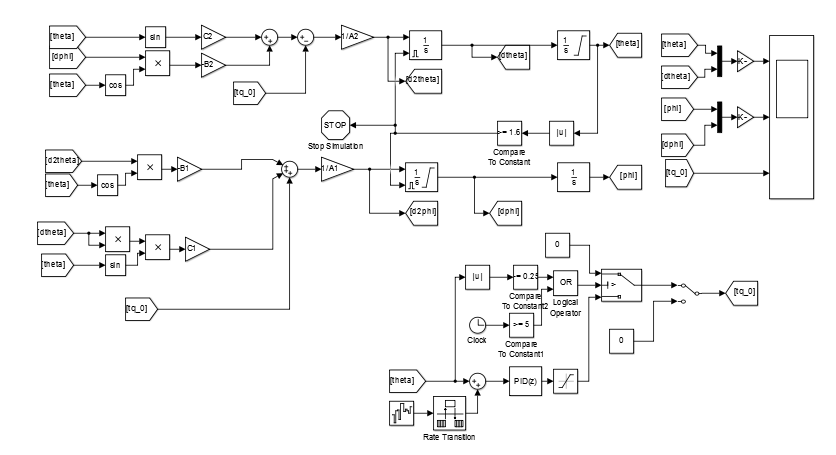
\includegraphics[scale=0.6]{sim_non_lin.PNG}
	\caption{Symulacja modelu nieliniowego}
	\label{fig:non_lin_sim}
\end{figure}

Przed każdym uruchomieniem można wybrać wartości początkowe podstawowych parametrów takich jak prędkość i pozycja kątowa koła oraz korpusu oraz nastawy regulatora i czas symulacji.
Parametry modelu ustawiane są w niezależnym skrypcie uruchamianym przed każdą symulacją. Po symulacji wykonywany jest skrypt wyrysowywujący przebiegi kluczowych zmiennych oraz prosta animacja wizualizująca przebieg symulacji.Pozwala to na szybką ocenę czy zachowanie modelu jest bliskie rzeczywistości. Przykładowy wynik symulacji został zaprezentowany na rysunku \ref{fig:non_lin_res} 

\begin{figure}[h]
	\centering
	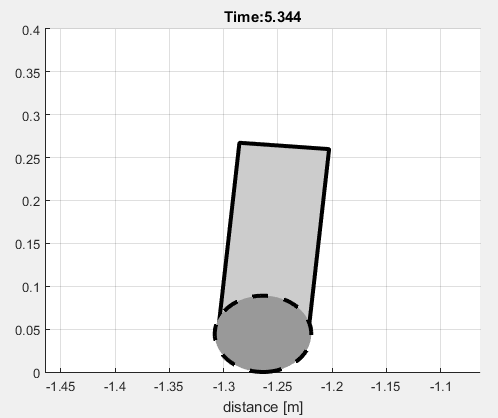
\includegraphics[scale=0.8]{visualisation_non_lin.PNG}
	\caption{Symulacja modelu nieliniowego}
	\label{fig:non_lin_res}
\end{figure}
\chapter{Sterowanie predykcyjne}
\label{cha:MPC}
Sterowanie predykcyjne (ang. MPC – model predictive control) to rodzaj sterowania w którym regulator dostosowuje swoje wyjście, nie tylko do akutalnego stanu układu, lecz także do 
przewidywanych przyszłych trajektorii. Przewidywany stan jest wyznaczany na podstawie aktualnych wejść oraz równań stanu ukladu. Wyznaczanie sterowania polega na cyklicznym wyznaczaniu optymalnej trajektorii przy warunkach początkowych równych akutalnemu stanu obiektu. Pierwszy odcinek sekwencji sterowań jest podawany na wejście obiektu, następnię cała procedura zostaje powtórzona dla aktualnego stanu obiektu w celu wyznaczenia nowej trajektorii. [ta ksiazka od mpc]. Przykładowy schemat obrazujący pracę regulatora predykcyjnego został przedstawiony na rysunku X.

-Wyjaśnienie symobli-

\section{Sterowanie predykcyjne na podstawie równań stanu}
\label{mpc_ss}

Dla uproszczenia podstawy matematyczne kontroli predykcyjnej zaprezentowane zostaną na prostym modelu z jednym wejściem i jednym wyjśćiem przedstawionym równaniami \ref{5row1}:\ref{5row1__1}

\begin{equation}
\label{5row1} 
x_m(k+1)=A_mx_m(k)+B_mu(k)
\end{equation}
\begin{equation}
\label{5row1__1} 
y(k)=C_mx_m(k)
\end{equation}

Gdzie $u$ jest wejściem systemu, $y$ to wyjście procesu a $x_m$ jest wektorem stanu długości $n_1$. Na potrzeby kontroli predykcyjnej konieczne będzie zapisanie systemu w postaci różnicowej \ref{5row2}

\begin{equation}
\label{5row2} 
\Delta x_m(k+1)=A_m\Delta x_m(k)+B_m\Delta u(k)
\end{equation}

Kolejnym etapem jest powiązanie $\Delta x_m(k)$ z wyjściem $y(k)$. Można to zrobić za pomocą nowego wektora stanu w postaci \ref{5row3}

\begin{equation}
\label{5row3} 
x(k)=[\Delta x_m(k)^T+y(k)]^T
\end{equation}

Wprowadzone przekształcenia pozwalają zapisać model \ref{5row1} w postaci rozszerzonej \ref{5row4}:\ref{5row5} będącej podstawą kontroli predykcyjnej. 
\begin{equation}
\label{5row4} 
x(k+1)=\begin{bmatrix}	A_m & o^T_m  \\	C_mA_m & 1 \end{bmatrix}
\begin{bmatrix}	\Delta x_m(k) \\y(k) \end{bmatrix}+
\begin{bmatrix}	B_m \\ C_mB_m \end{bmatrix} \Delta u(k)
\end{equation}
\begin{equation}
\label{5row5} 
y(k)=\begin{bmatrix}	o_m & 1 \end{bmatrix}  \begin{bmatrix} \Delta x_m(k) \\y(k) \end{bmatrix} 
\end{equation}


Uproszczony zapis postaci rozszerzonej został przedstawiony przy pomocy równań \ref{5row6}:\ref{5row7}


\begin{equation}
\label{5row6} 
x(k+1)=Ax(k)+B \Delta u(k)
\end{equation}
\begin{equation}
\label{5row7} 
y(k)=C \begin{bmatrix} \Delta x_m(k) \\y(k) \end{bmatrix} 
\end{equation}

\section{Kontrola predykcyjna z pojedyńczym oknem optymalizacji}

Po wprowadzeniu modelu rozszerzonego kolejnym etapem jest wyznaczenie przewidywanego wyjśćia obiektu na podstawie przyszłych wartości sterowania. Oszczacowanie to jest nazywane oknem optymalizacji. Parametrem definiującym okno jest jego długość $N_p$. Przyjmując, że w dyskretnej chwilę $k_i$ wektor $x(k_i)$ jest możliwy do pomiaru, stan $x(k_i)$ dostarcza informację o aktualnym stanie modelu. Trajektora przyszłych sterowań może zostać zapisana jako \ref{5row8}

\begin{equation}
\label{5row8} 
\Delta(k_i),\Delta(k_i+1), ..., \Delta(k_i+N_c-1),
\end{equation}

gdzie $N_c$ to horyzont kontroli oznaczający ilość wyznaczanych przyszłych próbek sterowania. Na podstawie informacji $x(k_i)$ przyszłe zmienne stanu wyznaczane są dla $N_p$ próbek gdzie parametr $N_p$ oznacza horyzont predykcji. Horyzont kontroli musi być mniejszy od równy od horyzontu predykcji.
Przyszłe zmienne stanu można zapisać w postaci \ref{5row9}

\begin{equation}
\label{5row9} 
x(k_i+1|k_i),x(k_i+2|k_i),...,x(k_i+m|k_i),...,x(k_i+N_p|k_i),
\end{equation}

Gdzie $x(k_i+m|k_i)$ jest przewidywanym stanem zmiennej w chwili $k_i+m$ na podstawie stanu $x(k_i)$. Na podstawie równań stanu wprowadzonych w punkcie \label{mpc_ss} przyszłe zmienne stanu są obliczane sekwencyjnie przy wykorzystaniu parametrów kontrolnych \ref{5row10}


 \begin{gather}
 \label{5row10}
x(k_i+1|k_i)=Ax(k_i)+B\Delta u(k_i) \\
\nonumber x(k_i+2|k_i)=Ax(k_i+1)+B\Delta u(k_i+1) \\
\nonumber =A^2x(k_i)+AB\Delta u(k_i)+B\Delta u(k_i+1) \\
%pionowe kropki%
\nonumber x(k_i+N_p|k_i)=A^{N_p}x(k_i)+A^{N_p-1}B\Delta u(k_i)+A^{N_p-2}B\Delta u(k_i+1) \\
\nonumber + ... + A^{N_p -N_c}B\Delta u(k_i+N_c-1)
\end{gather}

Na podstawie przyszłych zmiennych stanu wyznaczane są przyszłe wyjścia \ref{5row11}


\begin{gather}
\label{5row11}
y(k_i+1|k_i)=CAx(k_i)+CB\Delta u(k_i) \\
\nonumber y(k_i+2|k_i)=CA^2x(k_i)+CAB\Delta u(k_i)+CB\Delta u(k_i+1) \\
%pionowe kropki%
\nonumber y(k_i+N_p|k_i)=CA^{N_p}x(k_i)+CA^{N_p-1}B\Delta u(k_i)+CA^{N_p-2}B\Delta u(k_i+1) \\
\nonumber + ... + CA^{N_p -N_c}B\Delta u(k_i+N_c-1)
\end{gather}

Kolejnym krokiem jest wprowadzenie wektorów $Y$ i $\Delta U$ \ref{5row12}


\begin{gather}
\label{5row12}
Y=\begin{bmatrix} y(k_i+1 |k_i) & y(k_i+2 |k_i) & y(k_i+3 |k_i) & ... & y(k_i+N_p |k_i) \end{bmatrix} ^T\\
\nonumber \Delta U= \begin{bmatrix} \Delta u(k_i) & \Delta u(k_i+1) &  \Delta u(k_i+2) & ... &  \Delta u(k_i+N_c-1) \end{bmatrix} ^T
\end{gather}

Dzięki wektorom $Y$ i $\Delta U$ możliwe jest zapisanie \ref{5row10} i \ref{5row11} w postaci  \ref{5row13}

\begin{gather}
\label{5row13}
Y=Fx(k_i)+ \Phi \Delta U
\end{gather}

Gdzie

\begin{gather}
\label{5row14}
F= \begin{bmatrix} CA & CA^2 & CA^3 & \dots & CA^{N_p}\end{bmatrix}^T \\
\nonumber \Phi =  \begin{bmatrix} CB & 0 & 0 \dots & 0 \\
CAB & CB & 0 & \dots & 0 \\
CA^2B & CAB & CB & \dots & 0 \\%pionowe kropki?%
CA^{N_p-1}B & CA^{N_p-2}B & CA^{N_p-3}B & \dots & CA^{N_p-N_c}B \end{bmatrix}
\end{gather}

\section{Optymalizacja}
\label{mpc_optym}
Dla sygnałru $r(k_i)$ reprezentującego wartość zadaną w chwili $k_i$, w zakresie horyzontu predykcji, celem regulatora predykcyjnego jest sprowadzić przewidywane wyjście, tak blisko jak to możliwe do wartości zadanej. Wartość zadana pozostaje stała w pojedyńczym oknie optymalizacji. Wektor optymalnych sterowań $\Delta U$ minimalizuje funkcję błędu \ref{5row16} pomiędzy wartością zadaną a przewidywanym wyjściem układu.

\begin{gather}
\label{5row15}
R^T_s= \begin{bmatrix} 1_2 & 1_2 & ... & 1_{N_p}\end{bmatrix} r(k_i) 
\end{gather}


\begin{gather}
\label{5row16}
J=(R_s-Y)^T(R_s-Y)+\Delta U^T \bar{R} \Delta U 
\end{gather}

Pierwszy część równania \ref{5row16} jest odpowiada za minimalizację błędu pomiędzy wyjściem obietku a wartością zadaną. Druga część odpowiada kosztom odpowiadającym sterowaniu. Wyeliminwanie tego elementu sprawi, że duże wartości $\Delta U$ nie będą pogarszały wartości funkcji celu.

Aby uzyskać wektor optymalnych sterowań należy znaleźć minimum $J$ przy użyciu \ref{5row13}. Równanie \ref{5row16} można wtedy zapisać w postaci \ref{5row17}

\begin{gather}
\label{5row17}
J=(R_s-Fx(k_i))^T(R_s-Fx(k_i))- 2\Delta U^T \Phi^T (R_s-Fx(k_i)) +\Delta U^T (\Phi^T \Phi + \bar{R}) \Delta U 
\end{gather}

Warunkiem koniecznym istnienia minimum $J$ jest wyrażony równaniem \ref{5row18}
\begin{gather}
\label{5row18}
\frac{dJ}{d\Delta U}=0
\end{gather}

Przy wykorzystaniu równania \ref{5row18} można wyznaczyć wektor optymalnych sterowań w postaci \ref{5row19}

\begin{gather}
\label{5row19}
\Delta U = (\Phi^T \Phi + \bar{R})^{-1} \Phi^T(R_s-Fx(k_i))
\end{gather}

Przy założeniu, że $(\Phi^T \Phi + \bar{R})^{-1}$ istnieje. Macierz $(\Phi^T \Phi + \bar{R})^{-1}$ zgodnie z nomenklaturą nazywamy Hessianem.

Związek wektora sterowań optymlanych z wektorem stanu oraz wartością zadaną przedstawia równanie \ref{5row20}

\begin{gather}
\label{5row20}
\Delta U = (\Phi^T \Phi + \bar{R})^{-1} \Phi^T(\bar{R_s}r(k_i)-Fx(k_i))
\end{gather}

\section{Kontrola Predykcyjna z ograniczeniami}

Przedstawiona w sekcji \ref{mpc_optym} metoda wyznaczania wektora sterowań optymalnych $\Delta U$ nie umożliwia implementacji ograniczeń którym podlegają zmienne stanu oraz sterowanie. W rzeczywistych systemach sterowania wartości fizyczne opisujące obiekt mają ograniczony zakres. W omawianym w rozdziale \ref{cha:model} modelu robota większość ograniczeń wynika z ograniczonej mocy zastosowanych silników. Ich nota katalogowa omówiona w rozdziale \ref{cha:KonstrukcjaMechaniczna} pozwala oszacować maksymalny moment obrotowy, przyśpieszenie oraz prędkość kątową. Sterowanie wyznaczające wartości poza zakresem nie będzie mogło być zrealizowane. W celu zachowania zgodności systemu sterowania z rzeczywistym obiektem wprowadzone zostaną ograniczenia.

Ograniczenia w postaci \ref{5row21} mogą określać maksymalny przyrost zmiennej podczas jednej iteracji lub całkowitą wartość zmiennej. 

\begin{gather}
\label{5row21}
 \Delta x^{min} \leq \Delta x(k) \leq \Delta x^{max}\\
\nonumber  x^{min} \leq  x(k) \leq  x^{max}
\end{gather}

Następnym krokiem po sformułowaniu równań w postaci \ref{5row21} jest wprowadzenie tych zależności do procesu wyznaczania optymalnego sterowania. Ograniczenia przyrostu zmiennej są prostsze do wprowadzenia ze względu na zastosowaną postać różnicową równań stanu. Ograniczenia przyrostowe dla wektora $X$ mozna przedstawić jako zalezność \ref{5row22} która może zostać zapisane pod postacią dwóch nierówności \ref{5row23}

\begin{gather}
\label{5row22}
\Delta X^{min} \leq \Delta X \leq \Delta X^{max}
\end{gather}
\begin{gather}
\label{5row23}
-\Delta X \leq \Delta X^{min} \\
\nonumber \Delta X \leq \Delta X^{max}
\end{gather}

Nierówności \ref{5row23} można zapisać w postaci macierzowej \ref{5row24}
\begin{gather}
\label{5row24}
\begin{bmatrix} - I \\ I \end{bmatrix} \Delta X \leq \begin{bmatrix} - \Delta X^{min} \\ \Delta X^{max} \end{bmatrix}
\end{gather}

Ograniczenia rzeczywistej wartości zmiennej wymagają drobnej modyfikacji. W celu ograniczenia zakresu wartości przyjomwanych przez zmienną w systemie przyrostowym, ograniczona musi zostać suma wszystkich elementów rozważanego wektora $\Delta X$ oraz wartości począkowej $x(k_0)$. Zamieniając macierze jednostkowe macierzą Toeplitza $T$ przedstawionej równaniem \ref{5row25}

\begin{gather}
\label{5row25}
\begin{bmatrix} 1 & 0 & 0 \\ 0 & 1 & 0 \\ 0 & 0 & 1 \end{bmatrix} \longrightarrow  \begin{bmatrix} 1 & 0 & 0 \\ 1 & 1 & 0 \\ 1 & 1 & 1 \end{bmatrix}
\end{gather}

Zapis ten w formie macierzowej przyjmuje postać \ref{5row26}

\begin{gather}
\label{5row26}
\begin{bmatrix} - T \\ T \end{bmatrix} \Delta X \leq \begin{bmatrix} -  X^{min} + x(k_0) \\ \ X^{max} -x(k_0) \end{bmatrix}
\end{gather}

Znając wartości $max, \Delta max, min$ oraz $ \Delta min$ dla każdej zmiennej można sformułować dla niej ograniczenia w postaci macierzowej \ref{5row24} oraz \ref{5row26}. Wszystkie ograniczenia mają postać nierówności liniowych. Hessian $(\Phi^T \Phi + \bar{R})^{-1}$ jest pozytywnie określony a funkcja kosztu $J$ jest kwadratowa. Spełniając powyższe założenia problem wyznaczenia optymalnego sterowania $\Delta U$ staje się standardowym zadaniem optymalizacji kwadratowej z ograniczeniami 


\chapter{Optymalizacja sterowania}
\label{cha:opt}

W rozdziale \ref{cha:MPC} sformułowane zostało zadanie optymalizacji kwadratowej z ograniczeniami, którego rozwiązanie pozwoli wyznaczyć finalne sterowanie robota. Rozdział bieżący przedstawia zastosowane podejście do rozwiązania przedstawionego zadania zarówno w symulacji zaimplementowanej w pakiecie Matlab Simulink oraz w rzeczywistym sterowniku robota. 


%s\section{Testy}
 pertinacia voluptaria.



% itd.
% \appendix
% \include{dodatekA}
% \include{dodatekB}
% itd.

\printbibliography
\end{document}
